\documentclass[10pt,a4paper]{article}

% =========================================================================
% Packages
% =========================================================================
\usepackage{iftex}
\ifxetex
  \usepackage{fontspec}
  \setmainfont{Twentieth-Century.ttf}[
    Path=File/Font/,
    BoldFont=Twentieth-Century.ttf,
    ItalicFont=Twentieth-Century.ttf,
    BoldItalicFont=Twentieth-Century.ttf
  ]
\else
  \usepackage[utf8]{inputenc}
  \usepackage[T1]{fontenc}
  \usepackage[scaled=0.92]{helvet}
  \renewcommand{\familydefault}{\sfdefault}
\fi
\usepackage{geometry}
\usepackage{graphicx}
\graphicspath{{Gambar/}}
\usepackage{amsmath,amssymb}
\usepackage{fancyhdr}
\usepackage{titlesec}
\usepackage{booktabs}
\usepackage{tabularx}
\usepackage{array}
\usepackage{caption}
\usepackage{subcaption}
\usepackage{algorithm}
\usepackage{algpseudocode}
\usepackage{hyperref}
\usepackage{microtype}
\usepackage{url}
\usepackage{cite}
\renewcommand\citepunct{], [}
\renewcommand\citedash{]--[}
\usepackage{float}
\usepackage{placeins}

% =========================================================================
% Page Geometry & Margins (JTRIK Standard: A4 Paper, Margins: 2.5 cm all sides)
% =========================================================================
\geometry{
  a4paper,
  top=2.5cm,
  bottom=2.5cm,
  left=2.5cm,
  right=2.5cm,
  headheight=45pt,
  headsep=12pt,
  footskip=22pt
}

% Paragraph settings: Justified, single space, compact spacing for <= 10 pages
\setlength{\parindent}{0pt}
\setlength{\parskip}{4pt}
\linespread{1.0}

% Float Spacing Adjustments
\setlength{\floatsep}{8pt plus 2pt minus 2pt}
\setlength{\textfloatsep}{10pt plus 2pt minus 2pt}
\setlength{\intextsep}{8pt plus 2pt minus 2pt}

% Hyperlink configuration (Non-colored citations & links per JTRIK / Mendeley standard)
\hypersetup{
  hidelinks
}

% =========================================================================
% Header & Footer Settings
% =========================================================================
\pagestyle{fancy}
\fancyhf{}
\fancyhead[L]{\fontsize{9pt}{11pt}\selectfont JURNAL TEKNOLOGI REKAYASA INFORMASI DAN KOMPUTER}
\fancyfoot[R]{\fontsize{9pt}{11pt}\selectfont\thepage}
\renewcommand{\headrulewidth}{0.4pt}
\renewcommand{\footrulewidth}{0pt}

% First page header
\fancypagestyle{firstpage}{
  \fancyhf{}
  \fancyhead[L]{%
    \begin{minipage}[c]{0.78\textwidth}
      {\fontsize{9.5pt}{12pt}\selectfont\textbf{JURNAL TEKNOLOGI REKAYASA INFORMASI DAN KOMPUTER}}\\[2pt]
      {\fontsize{8.5pt}{10.5pt}\selectfont E-ISSN: 2797-1724, DOI: 10.000/jtrik.v1i1.2026}\\[1pt]
      {\fontsize{8.5pt}{10.5pt}\selectfont Vol. 1 No. 1 2026 pp. 01--10}
    \end{minipage}%
  }
  \fancyhead[R]{%
    \begin{minipage}[c]{0.20\textwidth}
      \raggedleft
      \IfFileExists{Gambar/image1.png}{
\includegraphics[height=1.05cm]{image1.png}}{}
    \end{minipage}%
  }
  \fancyfoot[R]{\fontsize{9pt}{11pt}\selectfont\thepage}
  \renewcommand{\headrulewidth}{0.5pt}
  \renewcommand{\footrulewidth}{0pt}
}

% =========================================================================
% Section Headings Formatting
% Level 1: 14pt Bold
% Level 2: 12pt Bold
% Level 3: 10pt Bold
% =========================================================================
\titleformat{\section}
  {\fontsize{13pt}{16pt}\bfseries}{\thesection.}{0.5em}{}
\titlespacing*{\section}{0pt}{10pt}{3pt}

\titleformat{\subsection}
  {\fontsize{11pt}{14pt}\bfseries}{\thesubsection}{0.5em}{}
\titlespacing*{\subsection}{0pt}{7pt}{2pt}

\titleformat{\subsubsection}
  {\fontsize{10pt}{12pt}\bfseries}{\thesubsubsection}{0.5em}{}
\titlespacing*{\subsubsection}{0pt}{5pt}{2pt}

% Caption styles (9 pt / small)
\captionsetup{font={small},labelfont=bf,justification=centering}
\captionsetup[table]{position=top,skip=3pt}
\captionsetup[figure]{position=bottom,skip=4pt}

% =========================================================================
% Document Body
% =========================================================================
\begin{document}
\thispagestyle{firstpage}

% --- Article Title (20pt Bold) ---
{\fontsize{19pt}{23pt}\bfseries\raggedright Penerapan Hybrid Recommendation System dengan Content-Based Filtering dan Euclidean Distance untuk Rekomendasi Warna Lipstik\par}
\vspace{6pt}

% --- Authors (10pt Regular) ---
{\fontsize{10pt}{12pt}\selectfont Dinda Fitria Indriana$^{1*}$, Muhammad Rizka$^{2}$, Rahmad Hidayat$^{3}$\par}
\vspace{3pt}

% --- Affiliations (9pt) ---
{\fontsize{8.5pt}{11pt}\selectfont
$^{1,2,3}$ Jurusan Teknologi Informasi dan Komputer, Politeknik Negeri Lhokseumawe, Jl. Banda Aceh--Medan Km. 280,3 Buketrata, Lhokseumawe 24301, Indonesia\par}
\vspace{3pt}

% --- Corresponding Author (9pt) ---
{\fontsize{8.5pt}{11pt}\selectfont
*Corresponding Author: \href{mailto:dindaindriana0911@gmail.com}{dindaindriana0911@gmail.com}\par}
\vspace{3pt}

% --- Article Info (9pt) ---
{\fontsize{8.5pt}{11pt}\selectfont
\textbf{Article info:} Received August 15, 2026, Revised August 25, 2026, Accepted September 01, 2026\par}
\vspace{3pt}

% --- Open Access License (8pt) ---
{\fontsize{8pt}{10pt}\selectfont
This is an open access article under the \href{https://creativecommons.org/licenses/by-sa/4.0/}{CC BY-SA} license.\par
\vspace{2pt}
\IfFileExists{Gambar/image3.png}{
\includegraphics[height=0.45cm]{image3.png}}{%
  \IfFileExists{Gambar/template_eprotik_image1.png}{
\includegraphics[height=0.45cm]{template_eprotik_image1.png}}{}%
}\par}

\vspace{4pt}
\noindent\rule{\textwidth}{0.4pt}
\vspace{2pt}

% --- Abstrak (13pt Heading, 9.5pt Regular Content) ---
{\fontsize{13pt}{15pt}\bfseries Abstrak\par}
\vspace{3pt}

{\fontsize{9.5pt}{12pt}\selectfont
Pemilihan warna lipstik yang sesuai dengan karakteristik warna alami bibir umumnya masih dilakukan secara subjektif dan konvensional, sehingga diperlukan suatu sistem yang mampu memberikan rekomendasi secara otomatis, objektif, dan personal. Penelitian ini bertujuan untuk merancang dan membangun sistem rekomendasi warna lipstik berdasarkan citra bibir menggunakan pendekatan Deep Learning melalui model MobileNetV2 serta Hybrid Recommendation System. Alur penelitian mencakup deteksi landmark wajah menggunakan MediaPipe Face Mesh, segmentasi area bibir, ekstraksi fitur nilai rata-rata Red, Green, Blue (RGB), pelabelan otomatis berbasis K-Means Clustering ke dalam kategori Pinkish, Brownish, dan Dark, klasifikasi tipe bibir dengan MobileNetV2 melalui transfer learning, serta pemberian rekomendasi warna lipstik melalui perpaduan Rule-Based Filtering dan Content-Based Filtering berbasis Euclidean Distance. Hasil evaluasi pengujian menunjukkan bahwa model MobileNetV2 berhasil mengklasifikasikan tipe warna bibir dengan akurasi validasi sebesar 94,84\%. Pada sistem rekomendasi, pengujian terhadap basis data shade lipstik komersial berhasil menghasilkan rekomendasi Top-3 dengan rata-rata tingkat kemiripan sebesar 93,62\% pada rekomendasi pertama, 92,26\% pada rekomendasi kedua, dan 91,41\% pada rekomendasi ketiga. Dengan demikian, sistem yang dikembangkan terbukti akurat dan efektif dalam memberikan rekomendasi warna lipstik yang sesuai dengan karakteristik warna alami bibir pengguna.\par}

\vspace{4pt}
{\fontsize{9.5pt}{12pt}\selectfont\textbf{Kata Kunci:} Deep Learning, MobileNetV2, Hybrid Recommendation System, Content-Based Filtering, Euclidean Distance, K-Means Clustering, Rekomendasi Warna Lipstik.\par}

\vspace{3pt}
\noindent\rule{\textwidth}{0.4pt}
\vspace{4pt}

% =========================================================================
% Section 1: Introduction
% =========================================================================
\section{PENDAHULUAN}

Perkembangan industri kosmetik di Indonesia mengalami peningkatan yang sangat pesat seiring dengan tingginya kesadaran masyarakat terhadap penampilan diri dan perawatan kecantikan. Berdasarkan survei pasar konsumen di Indonesia, produk riasan bibir seperti lipstik, \textit{lip cream}, dan \textit{lip tint} menduduki kategori produk kosmetik yang paling banyak digunakan oleh wanita, dengan persentase penggunaan mencapai 80,4\% \cite{jakpat2025}. Lipstik tidak hanya berfungsi sebagai pewarna bibir untuk meningkatkan estetika wajah, tetapi juga menjadi elemen penting dalam mengekspresikan karakter dan rasa percaya diri pemakainya.

Meskipun produk lipstik sangat populer, proses pemilihan warna (\textit{shade}) lipstik yang tepat sering kali menjadi tantangan bagi konsumen. Karakteristik warna dasar bibir setiap individu bersifat unik dan sangat bervariasi. Penelitian ilmiah oleh Vergnaud dkk. menunjukkan bahwa warna alami bibir dipengaruhi oleh berbagai faktor fisiologis yang kompleks, seperti konsentrasi melanin, aliran hemoglobin, ketebalan stratum korneum, etnis, dan usia \cite{vergnaud2024lip, vergnaud2023measurement}. Perbedaan pigmen dasar ini menyebabkan satu produk lipstik yang sama dapat menghasilkan tampilan warna akhir yang sangat berbeda ketika diaplikasikan pada bibir orang yang berbeda. Hal tersebut diperkuat oleh penelitian Charton dkk. yang berhasil menyusun bagan warna bibir (\textit{lip colour chart}) multi-etnis dan membuktikan keragaman spektrum rona bibir manusia \cite{charton2026development}.

Sebagian besar konsumen masih memilih warna lipstik secara konvensional dan subjektif, misalnya dengan mencoba produk langsung menggunakan \textit{tester} di toko fisik atau hanya mengandalkan ulasan di media sosial. Metode konvensional ini memiliki risiko higienitas serta berpotensi menimbulkan ketidakcocokan warna saat bertransaksi daring. Sejumlah penelitian terdahulu telah mengkaji sistem rekomendasi produk kecantikan. Katariya dan Patel merancang model CNN untuk merekomendasikan produk kosmetik berdasarkan tipe dan rona warna kulit (\textit{skin tone}) \cite{katariya2025novel}. Selanjutnya, Gulati dkk. mengembangkan sistem BeautifAI yang memberikan rekomendasi riasan terpersonalisasi berdasarkan karakteristik wajah dan kebutuhan acara (\textit{occasion}) pengguna \cite{gulati2023beautifai}. Pada aspek komputasi rekomendasi, Pratama dkk. menerapkan metode \textit{Content-Based Filtering} untuk sistem rekomendasi kosmetik berbasis kemiripan atribut produk \cite{pratama2025sistem}. Meskipun demikian, sebagian besar penelitian terdahulu tersebut masih menggunakan warna kulit wajah secara umum atau atribut teks katalog sebagai parameter acuan. Belum ditemukan penelitian yang secara spesifik mengekstraksi dan mengklasifikasikan karakteristik warna alami bibir pengguna sebagai basis utama rekomendasi warna lipstik.

Pemanfaatan teknologi \textit{Computer Vision} dan \textit{Deep Learning} berbasis \textit{Convolutional Neural Network} (CNN) terbukti sangat andal dalam mengenali pola visual citra secara akurat \cite{szeliski2022computer, goodfellow2016deep, lecun2015deep}. Salah satu arsitektur CNN yang efisien untuk implementasi praktis adalah MobileNetV2, yang dirancang menggunakan \textit{inverted residuals} dan \textit{linear bottlenecks} sehingga berbobot komputasi ringan tanpa mengorbankan akurasi tinggi \cite{sandler2018mobilenetv2, howard2017mobilenets}. Untuk mengelompokkan data warna bibir yang belum memiliki label acuan, algoritma \textit{unsupervised learning} K-Means Clustering dapat digunakan untuk membentuk klasterisasi data berbasis kemiripan nilai warna RGB \cite{macqueen1967methods, pedregosa2011scikit}.

Dalam sistem rekomendasi, pendekatan tunggal seperti \textit{Rule-Based Filtering} efektif untuk menyaring kandidat berdasarkan batasan kategori tertentu, namun tidak fleksibel dalam mengukur derajat kedekatan gradasi warna \cite{ricci2015recommender}. Sebaliknya, \textit{Content-Based Filtering} berbasis metrik jarak geometri \textit{Euclidean Distance} mampu mengukur kedekatan fitur numerik secara kontinu dan presisi \cite{aggarwal2016recommender}. Oleh karena itu, penggabungan keduanya ke dalam \textit{Hybrid Recommendation System} menjadi solusi ideal. Penelitian ini bertujuan merancang dan membangun sistem rekomendasi warna lipstik berbasis citra bibir dengan menerapkan MediaPipe Face Mesh \cite{lugaresi2019mediapipe} untuk segmentasi bibir otomatis, ekstraksi nilai rata-rata RGB, klasterisasi K-Means, klasifikasi MobileNetV2 dengan \textit{transfer learning}, serta perpaduan \textit{Rule-Based} dan \textit{Content-Based Filtering} (Euclidean Distance) untuk menghasilkan Top-3 rekomendasi lipstik paling presisi.

% =========================================================================
% Section 2: Methods
% =========================================================================
\section{METODE PENELITIAN}

\subsection{Alur Penelitian dan Arsitektur Sistem}
Penelitian ini dilaksanakan melalui tahapan sistematis yang terbagi ke dalam fase pengolahan data, pelatihan model \textit{deep learning}, perancangan sistem rekomendasi hybrid, dan evaluasi performa sistem. Alur umum sistem rekomendasi warna lipstik berbasis citra bibir diilustrasikan pada Gambar \ref{fig:alur_sistem}.

\begin{figure}[htbp]
  \centering
  \IfFileExists{Gambar/skripsi_image28_bw.png}{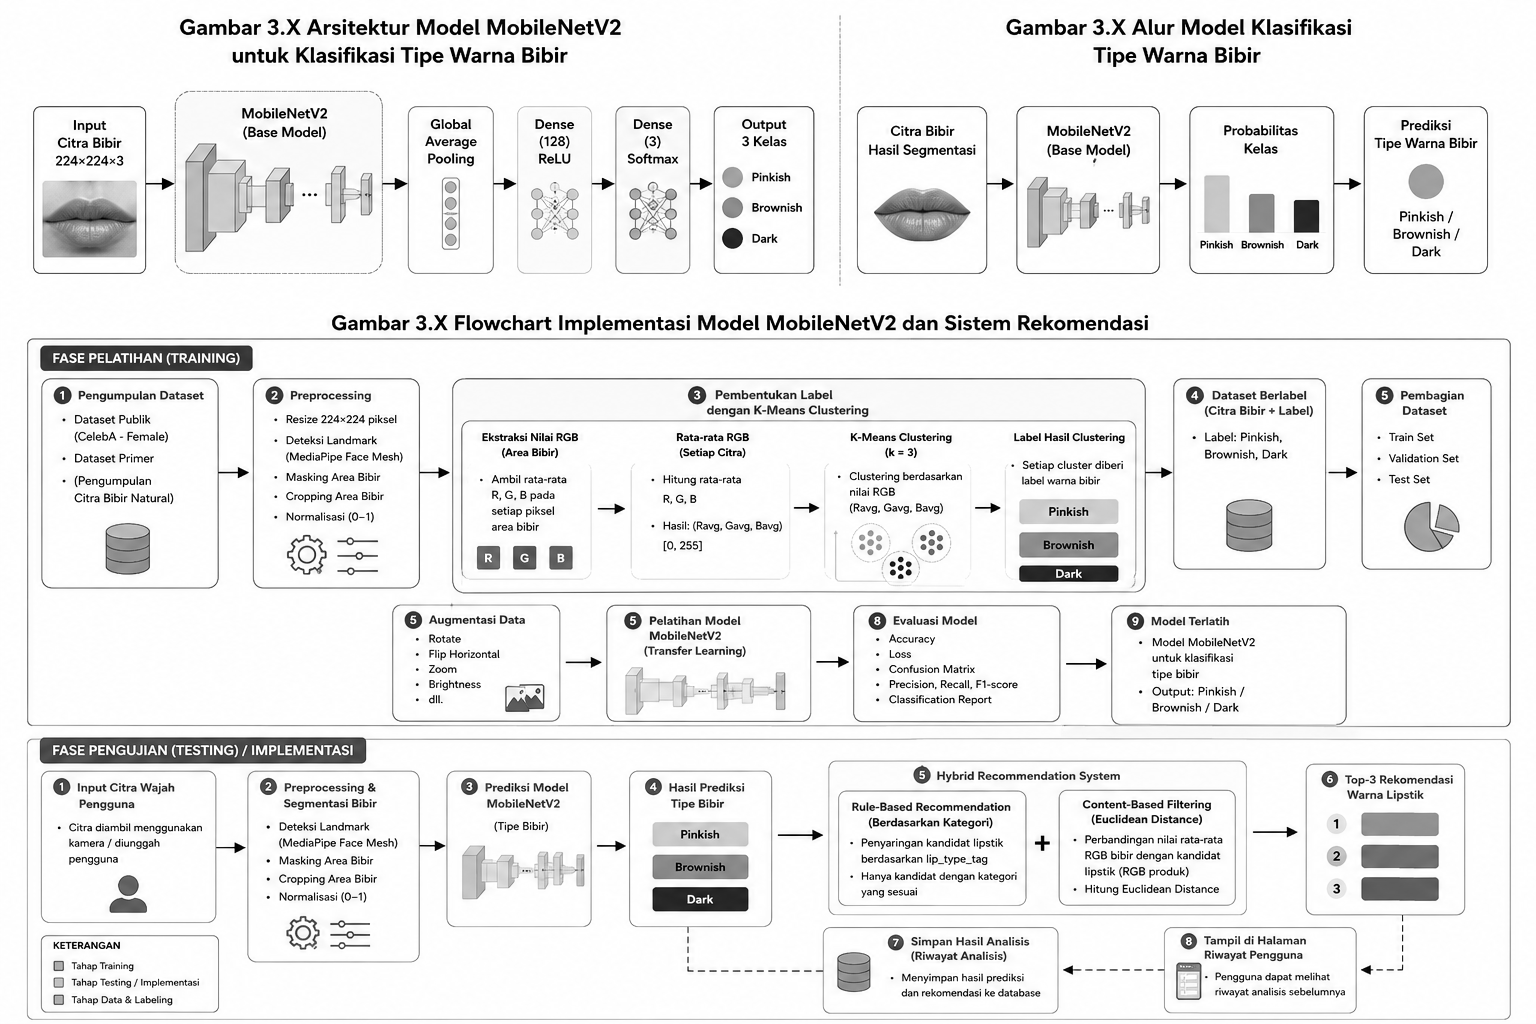
\includegraphics[width=0.72\textwidth]{skripsi_image28_bw.png}}{\fbox{Diagram Alur Sistem}}
  \caption{Diagram Alur Sistem Rekomendasi Warna Lipstik Menggunakan MobileNetV2 dan Hybrid Recommendation System}
  \label{fig:alur_sistem}
\end{figure}

\subsection{Pengumpulan dan Pembagian Dataset}
Dataset yang digunakan dalam penelitian ini berjumlah total 18.100 citra wajah, yang terdiri atas:
\begin{enumerate}
    \item Dataset Sekunder (CelebA): Sebanyak 18.000 citra wajah dari \textit{CelebFaces Attributes Dataset} (CelebA) \cite{liu2015deep} dengan ekspresi netral tanpa riasan bibir tebal.
    \item Dataset Primer: Sebanyak 100 citra wajah wanita Indonesia tanpa riasan bibir untuk meningkatkan representasi variasi pigmen bibir lokal.
\end{enumerate}
Dataset dibagi menjadi data latih (\textit{training set}) sebanyak 14.480 citra (80\%) dan data validasi (\textit{validation set}) sebanyak 3.620 citra (20\%) untuk pelatihan dan evaluasi model.

\subsection{Preprocessing dan Segmentasi Area Bibir}
Tahap \textit{preprocessing} bertujuan untuk mengekstraksi area bibir (\textit{Region of Interest} / ROI) dan menyeragamkan format citra:
\begin{enumerate}
    \item Resize Citra: Menyeragamkan ukuran citra masukan menjadi $224 \times 224$ piksel menggunakan OpenCV \cite{bradski2000opencv}.
    \item Deteksi Landmark Wajah: Menggunakan framework MediaPipe Face Mesh untuk mengekstrak 468 titik landmark wajah 3D \cite{lugaresi2019mediapipe}. Kontur bibir luar dan dalam diidentifikasi secara presisi (Gambar \ref{fig:landmark_seg}(a)).
    \item Segmentasi dan Masking: Membentuk masker poligon biner berdasarkan prinsip segmentasi citra digital \cite{otsu1979threshold, gonzalez2018digital} dari koordinat landmark bibir. Seluruh piksel di luar area bibir diatur bernilai nol (Gambar \ref{fig:landmark_seg}(b)).
    \item Normalisasi dan Cropping ROI: Mengonversi intensitas piksel kanal RGB ke rentang $[0, 1]$ dan memotong citra terfokus pada batas area bibir ($x_{\min}, y_{\min}, x_{\max}, y_{\max}$).
\end{enumerate}

\begin{figure}[htbp]
  \centering
  \begin{subfigure}[b]{0.46\textwidth}
    \centering
    \IfFileExists{Gambar/skripsi_image39_bw.png}{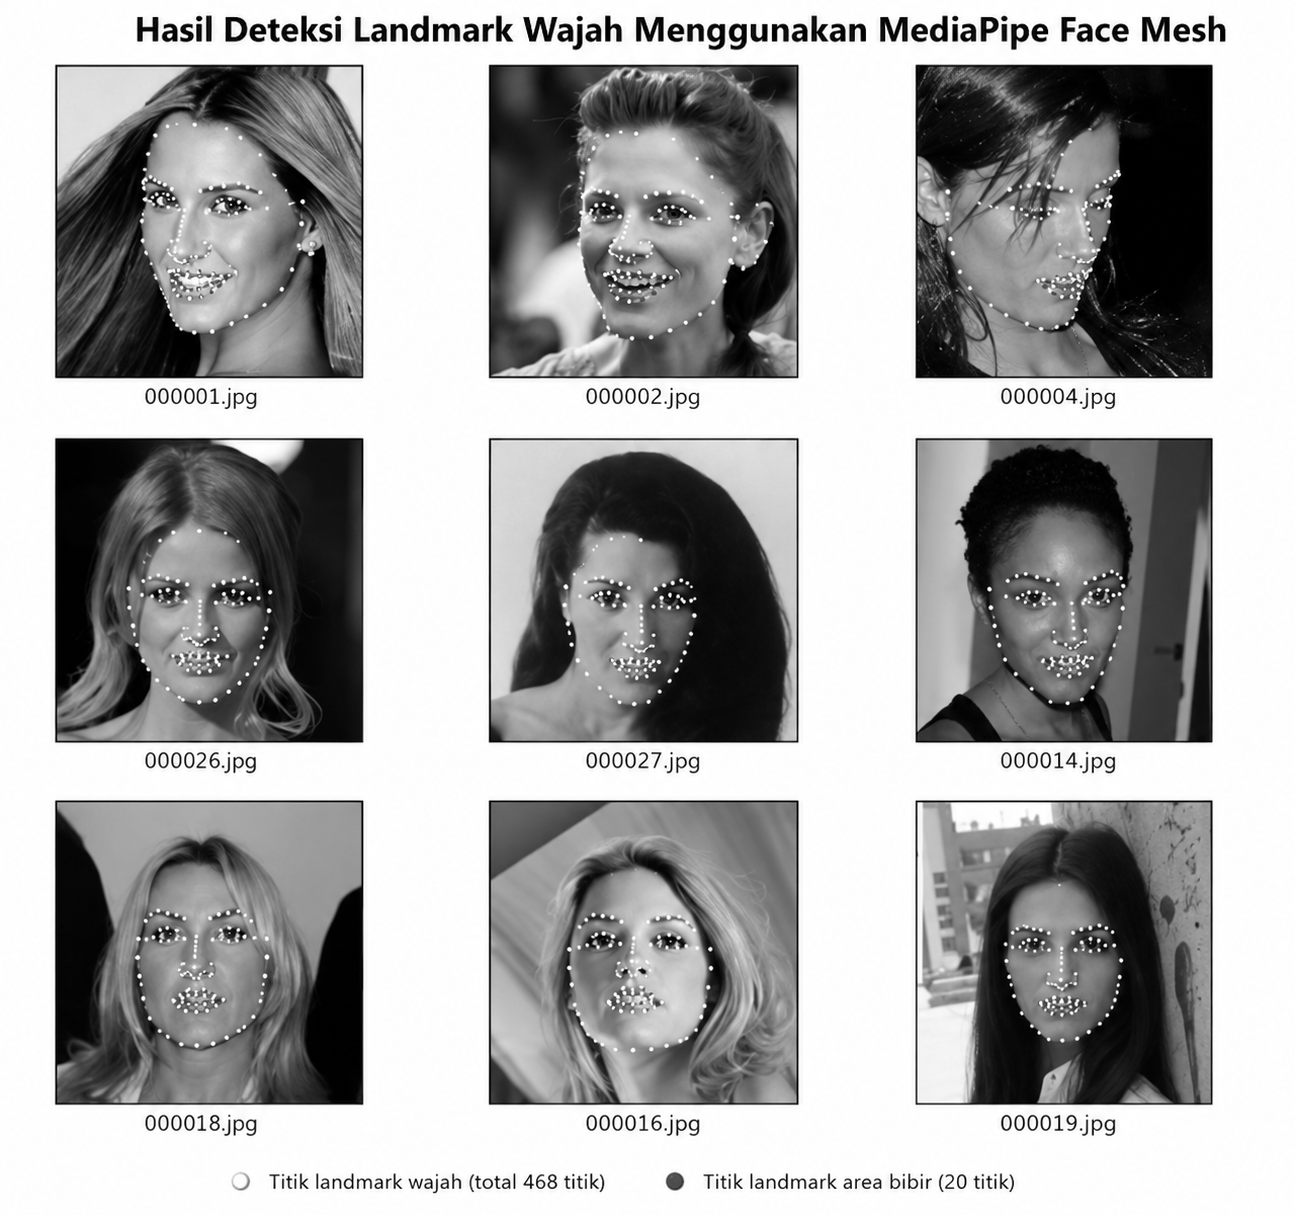
\includegraphics[width=\textwidth]{skripsi_image39_bw.png}}{\fbox{Landmark Wajah}}
    \caption{Deteksi Landmark MediaPipe}
    \label{fig:landmark}
  \end{subfigure}
  \hfill
  \begin{subfigure}[b]{0.46\textwidth}
    \centering
    \IfFileExists{Gambar/skripsi_image40_bw.png}{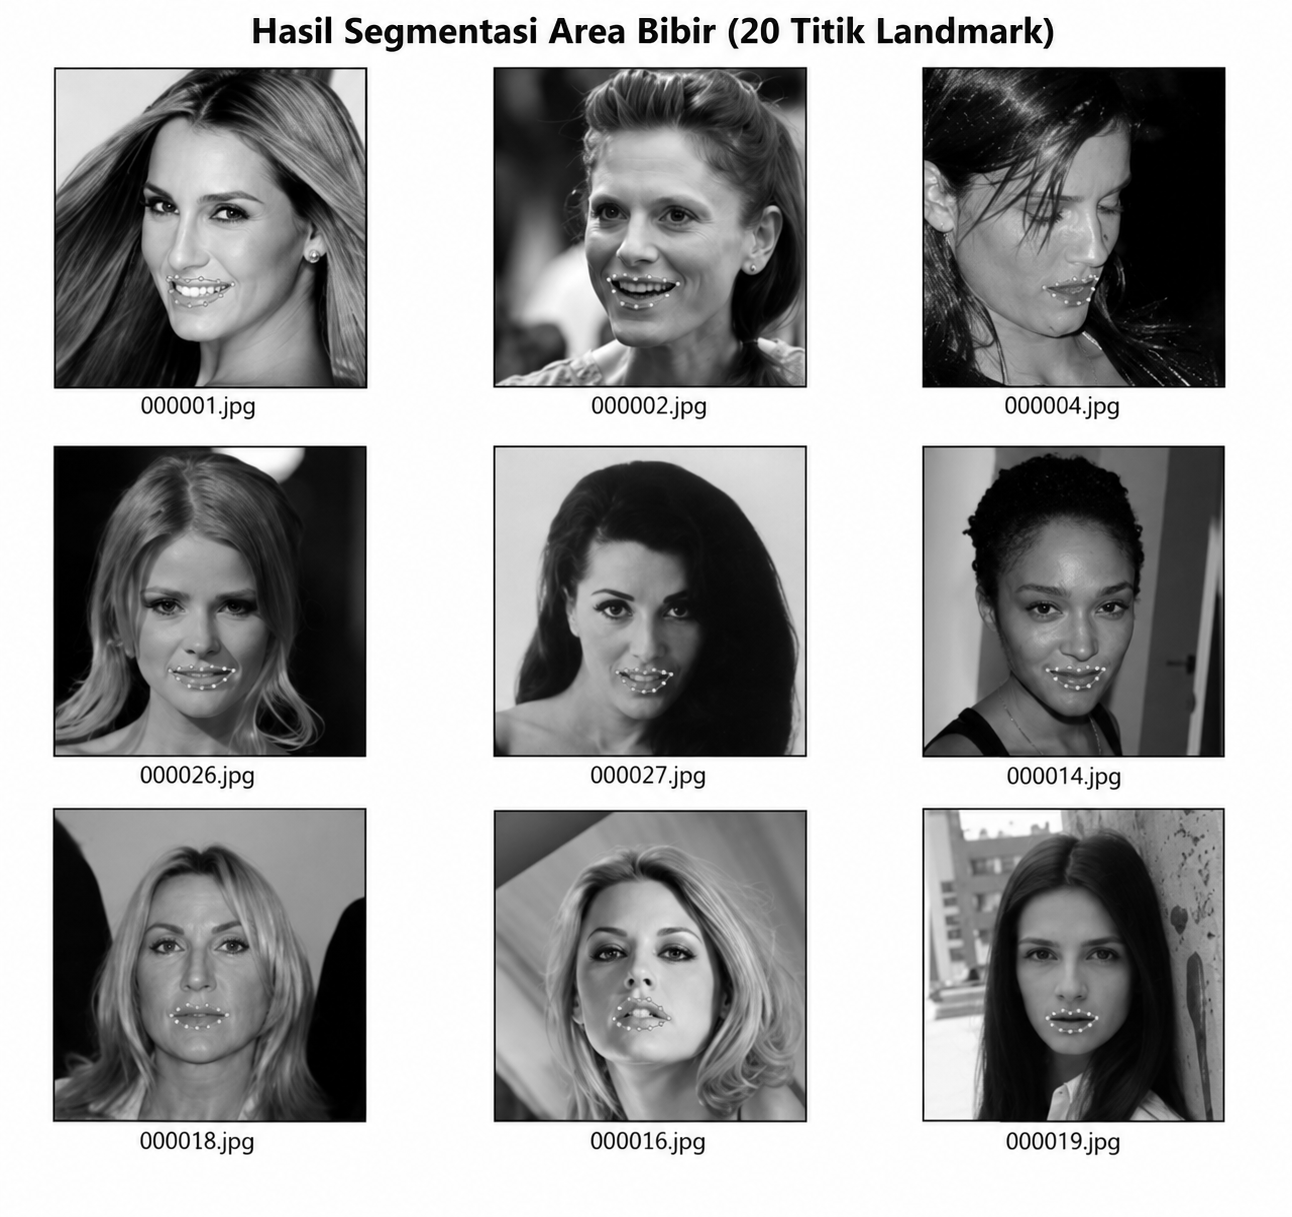
\includegraphics[width=\textwidth]{skripsi_image40_bw.png}}{\fbox{Segmentasi Bibir}}
    \caption{Segmentasi dan Masking Bibir}
    \label{fig:seg_bibir}
  \end{subfigure}
  \caption{Tahapan Deteksi Landmark Wajah dan Segmentasi Area Bibir Pengguna}
  \label{fig:landmark_seg}
\end{figure}

\subsection{Ekstraksi Fitur Warna dan K-Means Clustering}
Karakteristik warna bibir diekstraksi berdasarkan nilai rata-rata pada kanal Red ($R$), Green ($G$), dan Blue ($B$) dari seluruh $N$ piksel masker bibir menggunakan formula:
\begin{equation}
  \bar{R} = \frac{1}{N} \sum_{i=1}^N R_i, \quad \bar{G} = \frac{1}{N} \sum_{i=1}^N G_i, \quad \bar{B} = \frac{1}{N} \sum_{i=1}^N B_i
  \label{eq:rgb_avg}
\end{equation}

Tiga nilai skalar $(\bar{R}, \bar{G}, \bar{B})$ ini menjadi masukan algoritma K-Means Clustering ($K=3$, init \textit{k-means++}, random state 42) untuk menghasilkan 3 kategori label tipe bibir alami (Gambar \ref{fig:kmeans_viz}):
\begin{enumerate}
    \item Pinkish: Rona cerah dengan rona kemerahan/merah muda dominan ($\bar{R} > 150, \bar{G} \approx 95-120, \bar{B} \approx 100-125$).
    \item Brownish: Rona hangat kecokelatan ($\bar{R} \approx 125-155, \bar{G} \approx 75-100, \bar{B} \approx 65-90$).
    \item Dark: Rona bibir dengan pigmentasi gelap/pekat ($\bar{R} < 110, \bar{G} < 65, \bar{B} < 60$).
\end{enumerate}

\begin{figure}[htbp]
  \centering
  \IfFileExists{Gambar/skripsi_image44_bw.png}{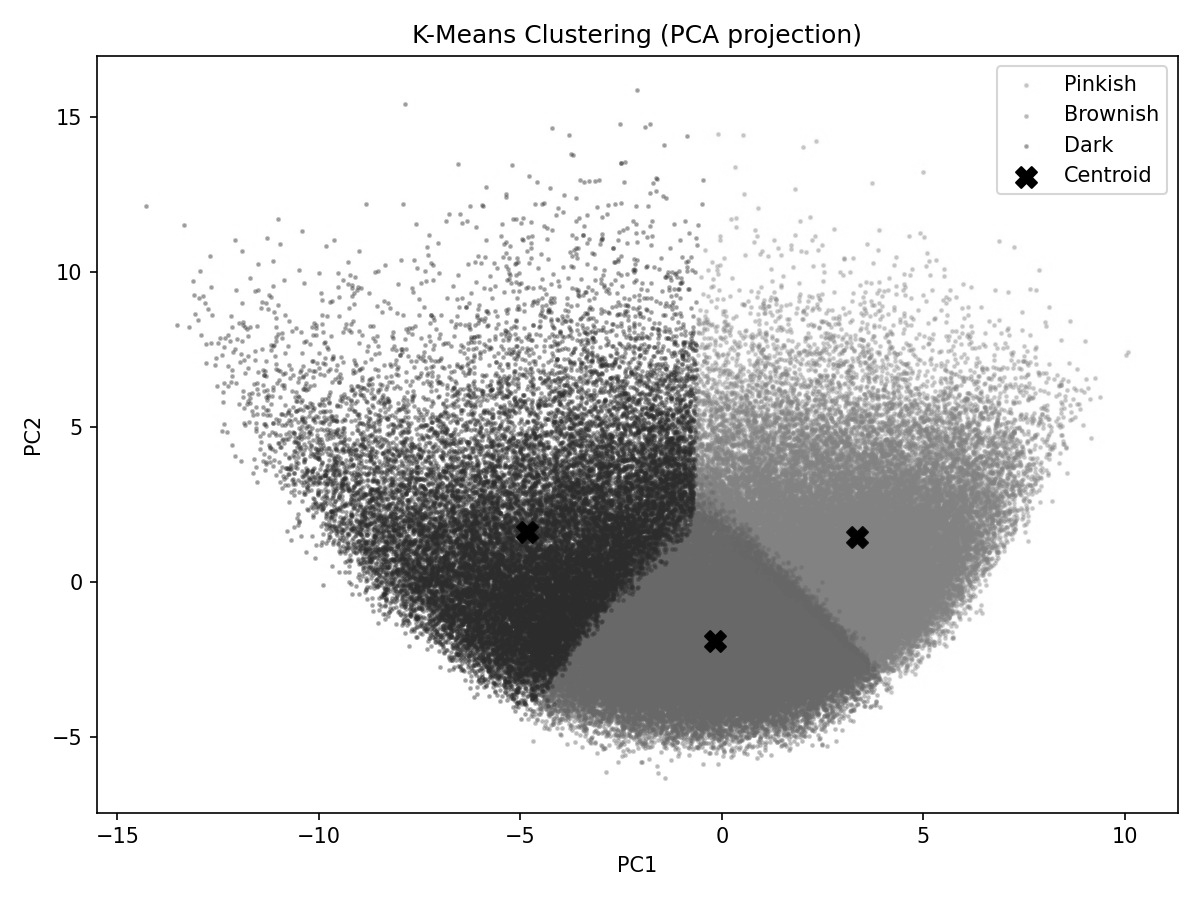
\includegraphics[width=0.48\textwidth]{skripsi_image44_bw.png}}{\fbox{Visualisasi K-Means}}
  \caption{Visualisasi Distribusi Hasil K-Means Clustering Warna Bibir ($K=3$)}
  \label{fig:kmeans_viz}
\end{figure}

\subsection{Pelatihan Model Klasifikasi MobileNetV2}
MobileNetV2 dilatih menggunakan pendekatan \textit{Transfer Learning} berbasis bobot ImageNet \cite{pan2010survey, he2016deep} yang didukung teknik augmentasi citra untuk memperluas variasi fitur \cite{shorten2019survey}. Lapisan kustom yang ditambahkan meliputi: \textit{Global Average Pooling 2D}, \textit{Dropout} (0.3), \textit{Dense} (128 neuron, ReLU), \textit{Dropout} (0.2), dan \textit{Dense Output} (3 neuron, Softmax). Konfigurasi parameter hiper pelatihan disajikan pada Tabel \ref{tab:param_pelatihan}.

\begin{table}[htbp]
  \centering
  \caption{Parameter Hiper Pelatihan Model MobileNetV2}
  \label{tab:param_pelatihan}
  \fontsize{8.5pt}{11pt}\selectfont
  \begin{tabular}{ll}
    \toprule
    \textbf{Parameter} & \textbf{Nilai / Konfigurasi} \\
    \midrule
    Arsitektur Dasar & MobileNetV2 (Pre-trained ImageNet) \\
    Dimensi Masukan Citra & $224 \times 224 \times 3$ piksel \\
    Jumlah Epoch & 30 \\
    Batch Size & 32 \\
    Optimizer & Adam ($\beta_1=0.9, \beta_2=0.999$, $\text{lr}=0.0001$) \\
    Fungsi Kerugian (Loss) & Categorical Crossentropy \\
    Jumlah Kelas Output & 3 (Pinkish, Brownish, Dark) \\
    \bottomrule
  \end{tabular}
\end{table}

\subsection{Hybrid Recommendation System}
Setelah model MobileNetV2 memprediksi probabilitas kelas tipe bibir pengguna ($\hat{y}_{\text{user}} \in \{\text{Pinkish}, \text{Brownish}, \text{Dark}\}$), sistem merekomendasikan shade lipstik terbaik melalui mekanisme bertingkat:

\subsubsection{Tahap 1: Rule-Based Filtering}
Sistem menyaring 281 koleksi lipstik komersial pada \textit{knowledge base} berdasarkan kesesuaian atribut \texttt{lip\_type\_tag} dengan kelas prediksi pengguna:
\begin{equation}
  \mathcal{C}_{\text{kandidat}} = \{ L_j \in \mathcal{D}_{\text{lipstik}} \mid \text{tag}(L_j) = \hat{y}_{\text{user}} \}
\end{equation}
Jumlah kandidat tersaring adalah 147 produk untuk Pinkish, 127 produk untuk Brownish, dan 14 produk untuk Dark (Tabel \ref{tab:rule_based}).

\begin{table}[htbp]
  \centering
  \caption{Aturan Rule-Based Recommendation Berdasarkan Tipe Warna Bibir}
  \label{tab:rule_based}
  \fontsize{8.5pt}{11pt}\selectfont
  \begin{tabular}{cllc}
    \toprule
    \textbf{No} & \textbf{Tipe Warna Bibir Prediksi} & \textbf{Kriteria Filter Knowledge Base} & \textbf{Jumlah Kandidat Produk} \\
    \midrule
    1 & Pinkish  & \texttt{lip\_type\_tag} = \textit{Pinkish}  & 147 produk \\
    2 & Brownish & \texttt{lip\_type\_tag} = \textit{Brownish} & 127 produk \\
    3 & Dark     & \texttt{lip\_type\_tag} = \textit{Dark}     & 14 produk \\
    \midrule
    \multicolumn{3}{l}{\textbf{Total Basis Data Lipstik}} & \textbf{281 produk} \\
    \bottomrule
  \end{tabular}
\end{table}

\subsubsection{Tahap 2: Content-Based Filtering Menggunakan Euclidean Distance}
Sistem menghitung jarak geometris ruang warna RGB (\textit{Euclidean Distance}) antara vektor warna bibir pengguna $\mathbf{u} = (R_u, G_u, B_u)$ dan warna lipstik $\mathbf{v}_j = (R_j, G_j, B_j)$ pada seluruh kandidat $L_j \in \mathcal{C}_{\text{kandidat}}$:
\begin{equation}
  d(\mathbf{u}, \mathbf{v}_j) = \sqrt{(R_u - R_j)^2 + (G_u - G_j)^2 + (B_u - B_j)^2}
  \label{eq:euclidean}
\end{equation}

Nilai jarak dikonversi menjadi persentase tingkat kemiripan (\textit{similarity score}) terhadap jarak maksimum ruang warna $d_{\max} = \sqrt{3 \times 255^2} \approx 441.673$:
\begin{equation}
  \text{Similarity}(\mathbf{u}, \mathbf{v}_j) = \left( 1 - \frac{d(\mathbf{u}, \mathbf{v}_j)}{d_{\max}} \right) \times 100\%
  \label{eq:similarity}
\end{equation}

Tiga produk dengan nilai \textit{similarity} tertinggi ditetapkan sebagai \textbf{Top-3 Lipstick Recommendation} (Algoritma \ref{alg:hybrid}).

\begin{algorithm}[htbp]
\caption{Algoritma Hybrid Recommendation System untuk Rekomendasi Lipstik}
\label{alg:hybrid}
\fontsize{8.5pt}{10.5pt}\selectfont
\begin{algorithmic}[1]
\Require Citra wajah pengguna $I_{\text{face}}$, Basis data produk lipstik $\mathcal{D}_{\text{lipstik}}$, Model klasifikasi MobileNetV2 $\mathcal{M}$.
\Ensure Tiga rekomendasi warna lipstik terbaik (Top-3) beserta nilai persentase kemiripan (\textit{similarity}).
\State $I_{\text{lip}} \gets \text{SegmentLipRegion}(I_{\text{face}})$ \Comment{Segmentasi MediaPipe Face Mesh}
\State $(R_u, G_u, B_u) \gets \text{ExtractAverageRGB}(I_{\text{lip}})$
\State $\hat{y}_{\text{user}} \gets \mathcal{M}.\text{predict}(I_{\text{lip}})$ \Comment{Klasifikasi: Pinkish, Brownish, atau Dark}
\State $\mathcal{C}_{\text{kandidat}} \gets \emptyset$
\For{each $L_j \in \mathcal{D}_{\text{lipstik}}$} \Comment{Tahap 1: Rule-Based Filtering}
    \If{$L_j.\text{tag} == \hat{y}_{\text{user}}$}
        \State $\mathcal{C}_{\text{kandidat}} \gets \mathcal{C}_{\text{kandidat}} \cup \{L_j\}$
    \EndIf
\EndFor
\State $\mathcal{R} \gets []$
\For{each $L_j \in \mathcal{C}_{\text{kandidat}}$} \Comment{Tahap 2: Content-Based Filtering}
    \State $(R_j, G_j, B_j) \gets L_j.\text{rgb}$
    \State $d_j \gets \sqrt{(R_u - R_j)^2 + (G_u - G_j)^2 + (B_u - B_j)^2}$
    \State $S_j \gets (1 - d_j / 441.673) \times 100\%$
    \State Append $(L_j, d_j, S_j)$ to $\mathcal{R}$
\EndFor
\State Sort $\mathcal{R}$ ascending by distance $d_j$
\State \Return Top-3 elements of $\mathcal{R}$
\end{algorithmic}
\end{algorithm}

\subsection{Metrik Evaluasi Performa}
Performa klasifikasi dievaluasi menggunakan matriks konfusi (\textit{Confusion Matrix}) serta metrik standar: \textit{Accuracy}, \textit{Precision}, \textit{Recall}, dan \textit{F1-Score} \cite{powers2011evaluation}:
\begin{equation}
  \text{Accuracy} = \frac{TP + TN}{TP + TN + FP + FN}
\end{equation}
\begin{equation}
  \text{Precision} = \frac{TP}{TP + FP}, \quad \text{Recall} = \frac{TP}{TP + FN}, \quad \text{F1-Score} = 2 \times \frac{\text{Precision} \times \text{Recall}}{\text{Precision} + \text{Recall}}
\end{equation}

% =========================================================================
% Section 3: Results and Discussion
% =========================================================================
\section{HASIL DAN PEMBAHASAN}

\subsection{Hasil Pelatihan dan Evaluasi Model MobileNetV2}
Model MobileNetV2 dilatih selama 30 epoch menggunakan dataset berlabel hasil klasterisasi K-Means. Gambar \ref{fig:eval_mobilenet}(a) menyajikan grafik konvergensi akurasi dan kerugian (\textit{loss}), sedangkan Gambar \ref{fig:eval_mobilenet}(b) menyajikan \textit{Confusion Matrix} hasil pengujian pada data validasi (803 sampel).

\begin{figure}[htbp]
  \centering
  \begin{subfigure}[b]{0.52\textwidth}
    \centering
    \IfFileExists{Gambar/skripsi_image45_bw.png}{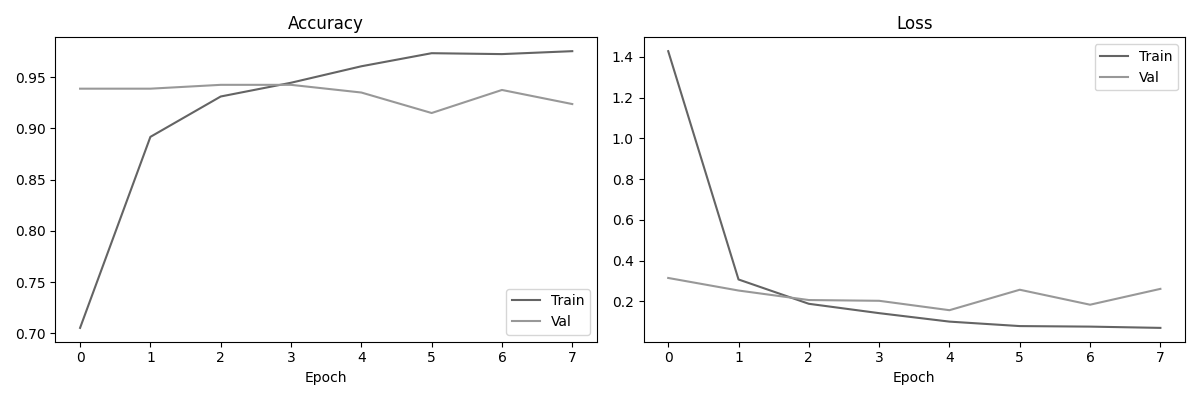
\includegraphics[width=\textwidth]{skripsi_image45_bw.png}}{\fbox{Grafik Akurasi dan Loss}}
    \caption{Grafik Akurasi dan Loss Pelatihan}
    \label{fig:loss_acc}
  \end{subfigure}
  \hfill
  \begin{subfigure}[b]{0.44\textwidth}
    \centering
    \IfFileExists{Gambar/skripsi_image46_bw.png}{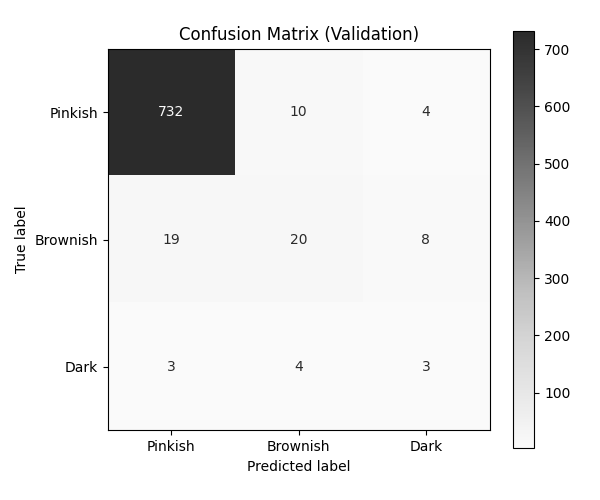
\includegraphics[width=\textwidth]{skripsi_image46_bw.png}}{\fbox{Confusion Matrix}}
    \caption{Confusion Matrix Data Validasi}
    \label{fig:cm}
  \end{subfigure}
  \caption{Evaluasi Performa Model MobileNetV2: (a) Grafik Akurasi dan Loss, (b) Confusion Matrix pada Data Validasi}
  \label{fig:eval_mobilenet}
\end{figure}

Model mencapai konvergensi stabil pada epoch ke-15 ke atas tanpa gejala \textit{overfitting}, dengan akurasi validasi akhir sebesar \textbf{94,84\%} dan \textit{validation loss} sebesar \textbf{0,1612}. Rincian nilai metrik evaluasi per kelas dirangkum dalam \textit{Classification Report} pada Tabel \ref{tab:classification_report}.

\begin{table}[htbp]
  \centering
  \caption{Classification Report Performa Model MobileNetV2}
  \label{tab:classification_report}
  \fontsize{8.5pt}{11pt}\selectfont
  \begin{tabular}{lcccc}
    \toprule
    \textbf{Kelas Tipe Bibir} & \textbf{Precision} & \textbf{Recall} & \textbf{F1-Score} & \textbf{Support (Sampel)} \\
    \midrule
    Pinkish      & 0.971 (97.1\%) & 0.981 (98.1\%) & 0.976 (97.6\%) & 746 \\
    Brownish     & 0.588 (58.8\%) & 0.426 (42.6\%) & 0.494 (49.4\%) & 47  \\
    Dark         & 0.200 (20.0\%) & 0.300 (30.0\%) & 0.240 (24.0\%) & 10  \\
    \midrule
    \textbf{Overall Accuracy} & \multicolumn{3}{c}{\textbf{0.940 (94.0\%)}} & \textbf{803} \\
    \textbf{Macro Average}    & 0.586 & 0.569 & 0.570 & 803 \\
    \textbf{Weighted Average} & 0.939 & 0.940 & 0.938 & 803 \\
    \bottomrule
  \end{tabular}
\end{table}

Model menunjukkan performa klasifikasi sangat tinggi pada kelas \textbf{Pinkish} (F1-score 97,6\%). Pada kelas \textbf{Brownish} dan \textbf{Dark}, nilai F1-score masing-masing tercatat 49,4\% dan 24,0\%. Karakteristik ini dipengaruhi oleh dominasi citra rona cerah pada dataset publik (\textit{class imbalance}). Namun secara agregat \textit{weighted average}, model mencapai F1-score 93,8\% dan akurasi 94,0\%, membuktikan efektivitas MobileNetV2 dalam mengenali karakteristik visual bibir.

\subsection{Pengujian dan Evaluasi Hybrid Recommendation System}
Pengujian sistem rekomendasi dilakukan terhadap 30 data uji pengguna dengan variasi nilai RGB bibir yang berbeda. Sampel hasil pengujian disajikan pada Tabel \ref{tab:hasil_rekomendasi}, dan rekapitulasi performa dirangkum pada Tabel \ref{tab:rekap_similarity}.

\begin{table}[htbp]
  \centering
  \caption{Sampel Hasil Pengujian Hybrid Recommendation System pada Data Uji Pengguna}
  \label{tab:hasil_rekomendasi}
  \fontsize{8.5pt}{10.5pt}\selectfont
  \begin{tabular}{ccclccc}
    \toprule
    \textbf{No} & \textbf{RGB User} & \textbf{Tipe Bibir} & \textbf{Rekomendasi Shade} & \textbf{RGB Lipstik} & \textbf{Euclidean ($d$)} & \textbf{Similarity (\%)} \\
    \midrule
    1 & (164, 121, 108) & Pinkish  & 1. Glossy Berry     & (167, 97, 101)  & 25.18 & 94.3\% \\
      &                 &          & 2. Dusty Rose       & (185, 115, 125) & 27.68 & 93.7\% \\
      &                 &          & 3. Cozy Cherry      & (173, 98, 94)   & 28.39 & 93.6\% \\
    \midrule
    2 & (128, 102, 99)  & Brownish & 1. Chilled Raspberry& (134, 85, 109)  & 20.62 & 95.3\% \\
      &                 &          & 2. Chilled Cranberry& (132, 68, 82)   & 38.22 & 91.3\% \\
      &                 &          & 3. Matte Berry      & (162, 83, 86)   & 41.06 & 90.7\% \\
    \midrule
    3 & (145, 98, 55)   & Pinkish  & 1. Satin Vermillion & (173, 95, 86)   & 41.88 & 90.5\% \\
      &                 &          & 2. Bold Ruby        & (176, 88, 86)   & 44.97 & 89.8\% \\
      &                 &          & 3. Cozy Cherry      & (173, 98, 94)   & 48.01 & 89.1\% \\
    \midrule
    4 & (195, 167, 153) & Brownish & 1. Mauve Bliss      & (170, 110, 130) & 66.36 & 85.0\% \\
      &                 &          & 2. Warm Terracotta  & (180, 105, 95)  & 74.35 & 83.2\% \\
      &                 &          & 3. Rose Brown       & (160, 95, 110)  & 81.12 & 81.6\% \\
    \bottomrule
  \end{tabular}
\end{table}

\begin{table}[htbp]
  \centering
  \caption{Rekapitulasi Skor Kemiripan (\textit{Similarity}) Hybrid Recommendation System}
  \label{tab:rekap_similarity}
  \fontsize{8.5pt}{11pt}\selectfont
  \begin{tabular}{lc}
    \toprule
    \textbf{Parameter Evaluasi} & \textbf{Nilai Kuantitatif} \\
    \midrule
    Jumlah Sampel Data Uji & 30 data \\
    Rata-rata Similarity Top-1 (Rekomendasi Pertama) & \textbf{93.62\%} \\
    Rata-rata Similarity Top-2 (Rekomendasi Kedua)   & \textbf{92.26\%} \\
    Rata-rata Similarity Top-3 (Rekomendasi Ketiga)  & \textbf{91.41\%} \\
    Nilai Similarity Tertinggi                      & \textbf{97.60\%} \\
    Nilai Similarity Terendah                       & \textbf{73.60\%} \\
    Total Basis Data Produk Lipstik Terdaftar       & 281 shade \\
    \bottomrule
  \end{tabular}
\end{table}

Hasil rekapitulasi membuktikan bahwa sistem rekomendasi hibrida mampu menghasilkan rekomendasi warna lipstik dengan tingkat kecocokan yang sangat tinggi. Rata-rata kemiripan warna untuk rekomendasi utama (Top-1) mencapai \textbf{93,62\%}, dengan seluruh Top-3 rekomendasi konsisten berada di atas 91\%. Pendekatan bertingkat (\textit{two-stage hybrid}) terbukti efektif mengeliminasi ketidakcocokan kategori pada tahap \textit{Rule-Based} dan mengoptimalkan presisi gradasi warna pada tahap \textit{Euclidean Distance}.

\subsection{Implementasi Antarmuka Sistem Berbasis Web}
Sistem diimplementasikan ke dalam aplikasi web responsif. Pengguna dapat mengunggah foto wajah dan sistem secara otomatis menampilkan ROI bibir tersegmentasi, nilai RGB, kelas prediksi MobileNetV2, nilai kepercayaan (\textit{confidence}), serta kartu Top-3 rekomendasi lipstik lengkap dengan swatch warna dan skor kemiripan (Gambar \ref{fig:ui_analisis}).

\begin{figure}[htbp]
  \centering
  \IfFileExists{Gambar/skripsi_image34_bw.png}{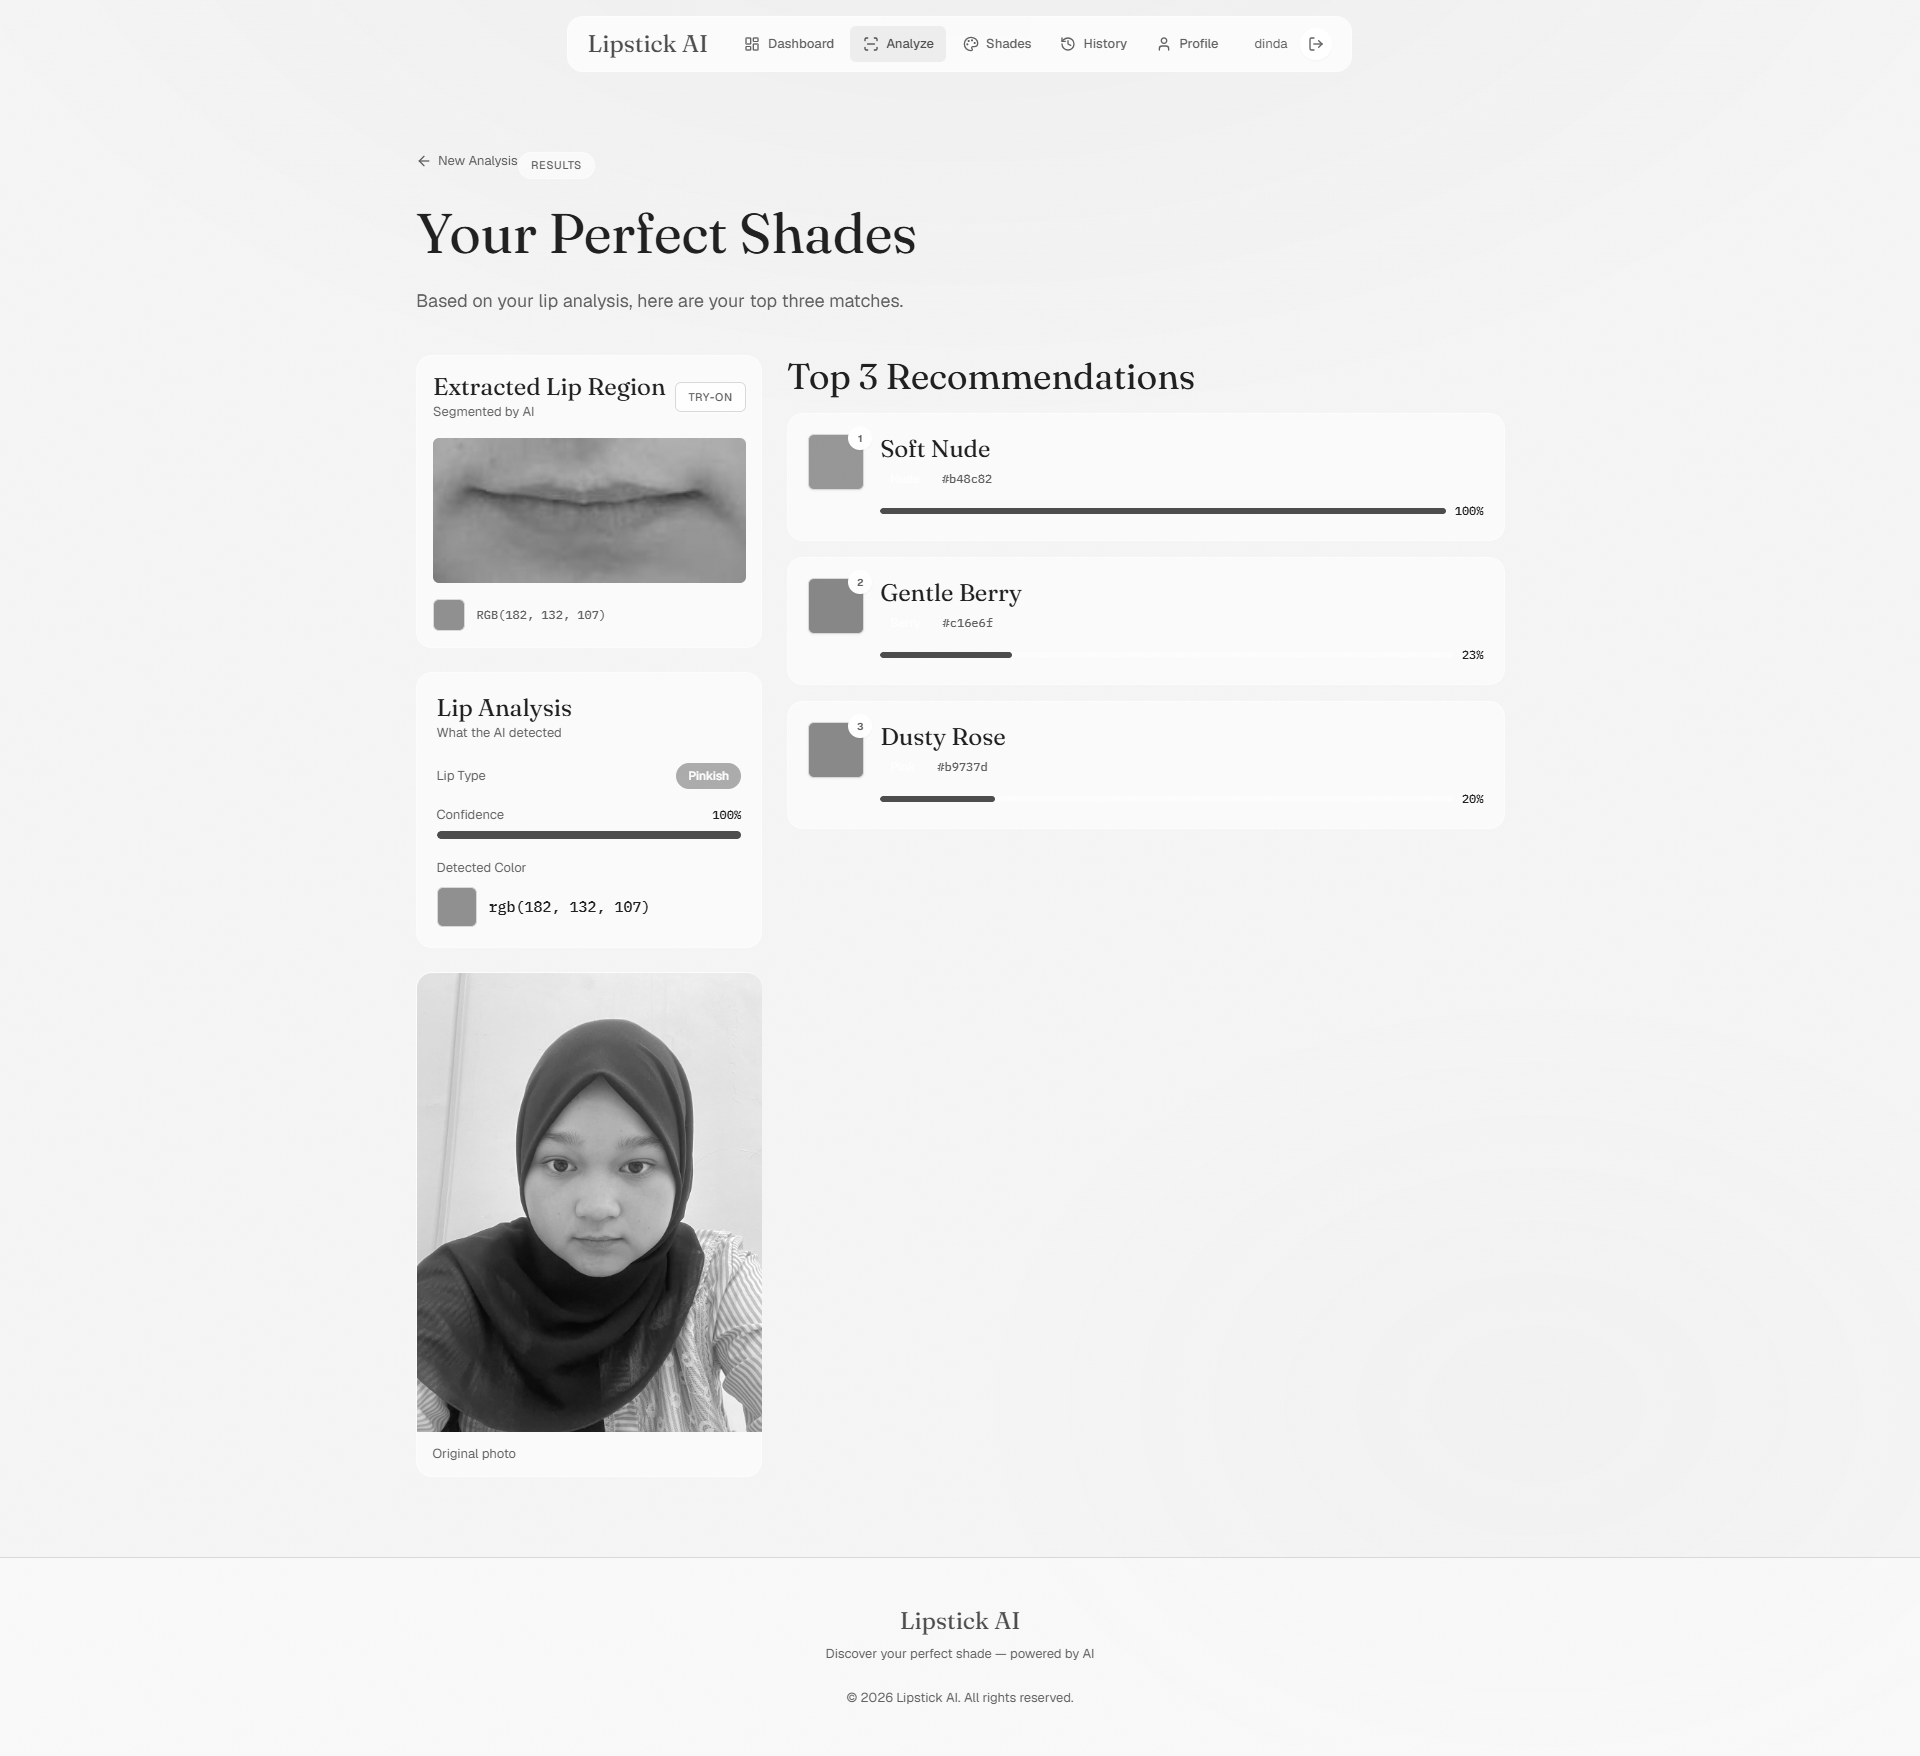
\includegraphics[width=0.55\textwidth]{skripsi_image34_bw.png}}{\fbox{Antarmuka Hasil Analisis}}
  \caption{Implementasi Antarmuka Halaman Hasil Analisis dan Rekomendasi Lipstik}
  \label{fig:ui_analisis}
\end{figure}

\subsection{Pengujian Fungsional (Black Box Testing)}
Pengujian fungsional sistem menggunakan metode \textit{Black Box Testing} menunjukkan bahwa seluruh modul aplikasi berjalan sesuai rancangan kebutuhan fungsional dengan status \textbf{100\% PASS} (Tabel \ref{tab:blackbox}).

\begin{table}[htbp]
  \centering
  \caption{Hasil Pengujian Black Box pada Modul Analisis dan Rekomendasi}
  \label{tab:blackbox}
  \fontsize{8pt}{10pt}\selectfont
  \begin{tabularx}{\textwidth}{clXXc}
    \toprule
    \textbf{No} & \textbf{Skenario Uji} & \textbf{Aktivitas / Masukan} & \textbf{Hasil yang Diharapkan} & \textbf{Status} \\
    \midrule
    1 & Unggah Citra Valid & Foto wajah JPG/PNG & Sistem mendeteksi wajah dan menampilkan \textit{preview} & PASS \\
    2 & Deteksi Landmark   & Menjalankan analisis & MediaPipe mengekstrak 468 titik landmark wajah & PASS \\
    3 & Segmentasi Bibir   & Ekstraksi batas bibir & Masker poligon bibir terbentuk dan area bibir terpotong & PASS \\
    4 & Klasifikasi Warna  & Ekstraksi RGB \& inferensi & MobileNetV2 memprediksi kelas (Pinkish/Brownish/Dark) & PASS \\
    5 & Rekomendasi Top-3  & Filter aturan \& jarak Euclidean & Menampilkan 3 produk lipstik dengan similarity tertinggi & PASS \\
    6 & Simpan Riwayat     & Simpan ke basis data & Riwayat tersimpan dan dapat diakses pada menu \textit{History} & PASS \\
    \bottomrule
  \end{tabularx}
\end{table}

\FloatBarrier
% =========================================================================
% Section 4: Conclusion
% =========================================================================
\section{KESIMPULAN DAN SARAN}

\subsection{Kesimpulan}
Berdasarkan hasil perancangan, implementasi, dan pengujian yang telah dilaksanakan, penelitian ini telah berhasil membangun sistem rekomendasi warna lipstik terpersonalisasi berbasis citra bibir dengan mengintegrasikan MediaPipe Face Mesh, MobileNetV2 melalui \textit{transfer learning}, serta \textit{Hybrid Recommendation System}. Model MobileNetV2 terbukti andal dalam mengklasifikasikan tipe warna bibir pengguna ke dalam tiga kategori (Pinkish, Brownish, dan Dark) dengan perolehan akurasi validasi mencapai 94,84\% dan nilai kerugian validasi sebesar 0,1612. Selain itu, integrasi metode \textit{Rule-Based Filtering} dan \textit{Content-Based Filtering} berbasis \textit{Euclidean Distance} berhasil mengoptimalkan akurasi rekomendasi produk lipstik dari katalog komersial, menghasilkan rata-rata tingkat kemiripan sebesar 93,62\% pada rekomendasi pertama, 92,26\% pada rekomendasi kedua, dan 91,41\% pada rekomendasi ketiga, dengan skor kecocokan tertinggi mencapai 97,60\%. Pengujian fungsionalitas menggunakan metode \textit{Black Box Testing} juga membuktikan bahwa seluruh modul aplikasi web berjalan lancar dengan tingkat keberhasilan 100\%.

\subsection{Saran}
Untuk pengembangan dan penyempurnaan penelitian di masa mendatang, disarankan untuk memperbanyak jumlah sampel data primer terutama pada kategori berpigmen gelap (Dark) dan kecokelatan (Brownish), serta menerapkan metode penanganan ketidakseimbangan kelas seperti \textit{class weighting} atau SMOTE guna meningkatkan sensitivitas pada kelas minoritas. Di samping itu, penelitian lanjutan dapat memperluas kapabilitas sistem dengan menambahkan fitur simulasi riasan virtual (\textit{Virtual Try-On}) berbasis \textit{Augmented Reality} (AR) interaktif serta mempertimbangkan integrasi rona warna kulit (\textit{skin undertone}) dan preferensi kebutuhan acara agar hasil rekomendasi kosmetik menjadi semakin komprehensif dan adaptif.

% =========================================================================
% References (IEEE Style)
% =========================================================================
\section*{DAFTAR PUSTAKA}

\begingroup
\renewcommand{\section}[2]{}%
\begin{thebibliography}{99}
\fontsize{8pt}{10pt}\selectfont
\setlength{\itemsep}{2pt}
\setlength{\parskip}{0pt}

\bibitem{jakpat2025}
Jakpat Survey, ``Makeup Product Categories Used by Indonesian Women in 2025,'' \textit{Databoks Katadata}, 2025, [Online]. Available: https://databoks.katadata.co.id/en/consumer-durables-apparel/statistics/692e89e11c6f5/makeup-product-categories-used-by-indonesian-women-in-2025

\bibitem{vergnaud2024lip}
H. Vergnaud \textit{et al.}, ``Lip Color Diversity: An Intricate Study,'' \textit{Skin Research and Technology}, vol. 30, no. 2, p. e13583, Feb. 2024, doi: 10.1111/srt.13583.

\bibitem{vergnaud2023measurement}
H. Vergnaud \textit{et al.}, ``Lip Color Measurement: A New Hyperspectral Imaging Device,'' \textit{Skin Research and Technology}, vol. 29, no. 8, p. e13418, Aug. 2023, doi: 10.1111/srt.13418.

\bibitem{charton2026development}
Z. Charton \textit{et al.}, ``Development of a Lip Colour Chart Across Four Ethnicities,'' \textit{International Journal of Cosmetic Science}, vol. 48, no. 1, pp. 161--171, Feb. 2026, doi: 10.1111/ics.70004.

\bibitem{katariya2025novel}
R. Katariya and S. Patel, ``A Novel Strid CNN Model for Cosmetic Product Recommendation based on Skin Type and Tone,'' \textit{SSRG International Journal of Electrical and Electronics Engineering}, vol. 12, no. 5, pp. 1--12, May 2025, doi: 10.14445/23488379/IJEEE-V12I5P101.

\bibitem{gulati2023beautifai}
K. Gulati, G. Verma, M. Mohania, and A. Kundu, ``BeautifAI: Personalised Occasion-based Makeup Recommendation,'' in \textit{Proc. 14th Asian Conf. Mach. Learn. (ACML)}, PMLR, vol. 189, pp. 407--419, Dec. 2023.

\bibitem{pratama2025sistem}
R. Pratama, M. Ikhsan, and A. Fitri, ``Sistem Rekomendasi Produk Kosmetik Menggunakan Metode Content-Based Filtering Berbasis Website,'' \textit{Jurnal Rabit: Jurnal Teknologi dan Sistem Informasi Univ. Abdurrab}, vol. 10, no. 1, pp. 45--56, Jan. 2025, doi: 10.36341/rabit.v10i1.6371.

\bibitem{szeliski2022computer}
R. Szeliski, \textit{Computer Vision: Algorithms and Applications}, 2nd ed. Cham, Switzerland: Springer Nature, 2022, doi: 10.1007/978-3-030-34372-9.

\bibitem{goodfellow2016deep}
I. Goodfellow, Y. Bengio, and A. Courville, \textit{Deep Learning}. Cambridge, MA, USA: MIT Press, 2016.

\bibitem{lecun2015deep}
Y. LeCun, Y. Bengio, and G. Hinton, ``Deep Learning,'' \textit{Nature}, vol. 521, no. 7553, pp. 436--444, May 2015, doi: 10.1038/nature14539.

\bibitem{sandler2018mobilenetv2}
M. Sandler, A. Howard, M. Zhu, A. Zhmoginov, and L.-C. Chen, ``MobileNetV2: Inverted Residuals and Linear Bottlenecks,'' in \textit{Proc. IEEE/CVF Conf. Comput. Vis. Pattern Recognit. (CVPR)}, pp. 4510--4520, Jun. 2018, doi: 10.1109/CVPR.2018.00474.

\bibitem{howard2017mobilenets}
A. G. Howard \textit{et al.}, ``MobileNets: Efficient Convolutional Neural Networks for Mobile Vision Applications,'' \textit{arXiv preprint arXiv:1704.04861}, Apr. 2017, [Online]. Available: https://arxiv.org/abs/1704.04861

\bibitem{macqueen1967methods}
J. MacQueen, ``Some Methods for Classification and Analysis of Multivariate Observations,'' in \textit{Proc. 5th Berkeley Symp. Math. Statist. Prob.}, vol. 1, pp. 281--297, 1967.

\bibitem{pedregosa2011scikit}
F. Pedregosa \textit{et al.}, ``Scikit-learn: Machine Learning in Python,'' \textit{Journal of Machine Learning Research}, vol. 12, pp. 2825--2830, Nov. 2011.

\bibitem{ricci2015recommender}
F. Ricci, L. Rokach, and B. Shapira, \textit{Recommender Systems Handbook}, 2nd ed. New York, NY, USA: Springer, 2015, doi: 10.1007/978-1-4899-7637-6.

\bibitem{aggarwal2016recommender}
C. C. Aggarwal, \textit{Recommender Systems: The Textbook}. Cham, Switzerland: Springer Nature, 2016, doi: 10.1007/978-3-319-29659-3.

\bibitem{lugaresi2019mediapipe}
C. Lugaresi \textit{et al.}, ``MediaPipe: A Framework for Building Perception Pipelines,'' \textit{arXiv preprint arXiv:1906.08172}, Jun. 2019, [Online]. Available: https://arxiv.org/abs/1906.08172

\bibitem{liu2015deep}
Z. Liu, P. Luo, X. Wang, and X. Tang, ``Deep Learning Face Attributes in the Wild,'' in \textit{Proc. IEEE Int. Conf. Comput. Vis. (ICCV)}, pp. 3730--3738, Dec. 2015, doi: 10.1109/ICCV.2015.425.

\bibitem{bradski2000opencv}
G. Bradski, ``The OpenCV Library,'' \textit{Dr. Dobb's Journal of Software Tools}, vol. 25, no. 11, pp. 120--125, Nov. 2000.

\bibitem{otsu1979threshold}
N. Otsu, ``A Threshold Selection Method from Gray-Level Histograms,'' \textit{IEEE Transactions on Systems, Man, and Cybernetics}, vol. 9, no. 1, pp. 62--66, Jan. 1979, doi: 10.1109/TSMC.1979.4310076.

\bibitem{gonzalez2018digital}
R. C. Gonzalez and R. E. Woods, \textit{Digital Image Processing}, 4th ed. New York, NY, USA: Pearson, 2018.

\bibitem{pan2010survey}
S. J. Pan and Q. Yang, ``A Survey on Transfer Learning,'' \textit{IEEE Transactions on Knowledge and Data Engineering}, vol. 22, no. 10, pp. 1345--1359, Oct. 2010, doi: 10.1109/TKDE.2009.191.

\bibitem{he2016deep}
K. He, X. Zhang, S. Ren, and J. Sun, ``Deep Residual Learning for Image Recognition,'' in \textit{Proc. IEEE Conf. Computer Vision and Pattern Recognition (CVPR)}, pp. 770--778, Jun. 2016, doi: 10.1109/CVPR.2016.90.

\bibitem{shorten2019survey}
C. Shorten and T. M. Khoshgoftaar, ``A Survey on Image Data Augmentation for Deep Learning,'' \textit{Journal of Big Data}, vol. 6, no. 1, p. 60, Jul. 2019, doi: 10.1186/s40537-019-0197-0.

\bibitem{powers2011evaluation}
D. M. W. Powers, ``Evaluation: From Precision, Recall and F-Measure to ROC, Informedness, Markedness and Correlation,'' \textit{Journal of Machine Learning Technologies}, vol. 2, no. 1, pp. 37--63, Dec. 2011.

\end{thebibliography}
\endgroup

\end{document}
